%------------------
%	PRZEWODNIK PO UBUNTU 14.04 LTS TRUSTY THAR
%	
%
%	Autorzy:
%		1. Piotr "Dwimenor Vali" Sochocki, dwimeron@gmail.com
%
%	Licencja:
%		Creative Commons
%		Uznanie autorstwa-Uzycie niekomercyjne-Na tych samych warunkach 3.0 Polska
%		CC BY-NC-SA 3.0 PL
%		http://creativecommons.org/licenses/by-nc-sa/3.0/pl/
%------------------


%------------------
%	PREAMBUŁA
%------------------
%TODO użyj paczki menukeys wszędzie tam, gdzie każe się coś wcisnąć na klawiaturze.

% klasa mwart autorstwa Marcina Wolińskiego
% http://marcinwolinski.pl/mwcls.html
% pakiet: texlive-lang-polish
\documentclass[a4paper,11pt,oneside]{mwart}

% orientacja pozioma, marginesy
\usepackage[landscape, margin=0.5in]{geometry}

% interlinia (1.6 = półtora linni odstępu wg. nomenklatury Worda/Writera)
\linespread{1.6}

% Odległosć między akapitami
\setlength{\parskip}{0.2cm}

% Język polski, polfonty
\usepackage[OT4]{polski}
\usepackage[utf8]{inputenc}

% dzielenie wierszy
\brokenpenalty=1000
\clubpenalty=1000
\widowpenalty=1000

% Obrazki
\usepackage{graphicx}
\usepackage{wrapfig}

% linki, URL
\usepackage[urlcolor=blue, colorlinks=true]{hyperref} 

% Dwie kolumny w spisie treści
\usepackage[toc]{multitoc}

% Jako, że nie bawimy się w rozdziały, sekcja i podsekcja są podstawowymi jednostmaki podziału dokumentu.
% Poniższa komenda wymusza numerowanie sekcji od "1" zamiast od "0"
\renewcommand*\thesection{\arabic{section}}

% Gwizadka zamiast myślnika jak znak kolejnego punktu listy.
\renewcommand{\labelitemi}{$\star$}

% Oficjalne kolory Ubuntu
% http://design.ubuntu.com/brand/colour-palette
\usepackage{xcolor}
\definecolor{ubuntu_orange}{RGB}{221,72,20}

%------------------
%	STRUKTURA DOKUMENTU
%------------------
\begin{document}

\thispagestyle{empty}

%-----------------
%	TYTUŁ
%-----------------

\colorbox{ubuntu_orange}{
	\parbox[t]{1.0\linewidth}{
		\centering \fontsize{40pt}{70pt}\selectfont
		\vspace*{0.7cm}
		
		\hfill Przewodnik po\\
		\hfill Ubuntu 14.04 LTS\\
		\hfill Trusty Thar\par
		
		\vspace*{0.7cm}
	}
}

\vfill

%-----------------
%	AUTOR
%-----------------

{
	\centering
	\large 
	\hfill Zespół \href{http://www.ubuntu.pl}{ubuntu.pl} \\
}

%----------------------------------------------------------------------------------------

\clearpage
\input{spis_tresci}
\section{Wstęp}
	\noindent Witaj w \textcolor{ubuntu_orange}{Przewodniku po Ubuntu Linux 14.04 Trusty Tahr!}

Niniejszy dokument pomoże ci zainstalować oraz skonfigurować system operacyjny Ubuntu. Przewodnik obejmuje każdy etap procesu zmiany systemu, od przygotowania twoich plików i ustawień, po instalowanie oraz używanie świeżo zainstalowanej kopii Ubuntu.

Przewodnik ten został napisany z myślą o osobach nieposiadających wiedzy technicznej, a większość terminów technicznych opatrzono stosownymi objaśnieniami. Przewodnik zadaje także kłam mitowi, że używanie Linuksa wiąże się z koniecznością wpisywania niezrozumiałych komend w konsoli. Cały tekst został przygotowany z myślą o wykorzystaniu graficznych narzędzi dostarczanych wraz z systemem.

Mamy nadzieję, że dzięki lekturze tego przewodnika bezproblemowo zainstalujesz Ubuntu na swoim komputerze i będziesz zadowolony mogąc korzystać z darmowego oraz otwartego systemu operacyjnego.\\
Wersja Ubuntu, która została opisana w tym poradniku, nosi nazwę Ubuntu GNU/Linux 14.04 LTS Trusty Tahr, co oznacza:
\begin{itemize}
\item \textcolor{ubuntu_orange}{Ubuntu} ---  nazwa całej serii systemów operacyjnych wydawanych przez firmę Canonical;
\item \textcolor{ubuntu_orange}{GNU/Linux} --- system bazuje na jądrze Linux i wykorzystuje oprogramowanie GNU;
\item \textcolor{ubuntu_orange}{14.04} --- jest to wersja z kwietnia (04) 2014 roku;
\item \textcolor{ubuntu_orange}{LTS} --- jest to wersja o przedłużonym wsparciu technicznym, a poprawki będą wydawane do 2019 roku;
\item \textcolor{ubuntu_orange}{Trusty Tahr} --- nazwa kodowa tego wydania.
\end{itemize}

	\subsection{O Ubuntu}
		Ubuntu jest kompletnym systemem operacyjnym utrzymywanym i rozwijanym przez firmę Canonical. Pierwsza jego wersja ukazała się w 2004 roku, a w ciągu 10 lat system ten zdobył rzesze fanów. Ubuntu wraz ze swoimi odmianami jest najpopularniejszą na świecie dystrybucją Linuksa. Samo słowo Ubuntu w języku afrykańskiego plemienia Zulusów oznacza ,,człowieczeństwo wobec innych'', w kontekście systemu operacyjnego tłumaczone jest jednak jako ,,Linux dla ludzi''.

Ideą systemu Ubuntu jest dostarczenie użytkownikowi kompletnego systemu operacyjnego, zawierającego wszystkie elementy niezbędne do codziennej pracy, a jednocześnie umożliwiającego posiadaczowi komputera swobodne korzystanie z systemu i modyfikowanie poszczególnych jego elementów. Wybierając Ubuntu nie musisz się zastanawiać nad tym, czy twój procesor nie ma przypadkiem zbyt dużej liczby rdzeni, co w przypadku korzystania z systemu komercyjnego mogłoby wymagać zakupu innej licencji. Nie musisz się również przejmować tym, że w firmie masz dziesięć komputerów, a twoja licencja na pakiet biurowy pozwala na instalację jedynie na sześciu stanowiskach. Jeśli chodzi o to, jak i do czego wykorzystasz system i oprogramowanie, wszystko zależy wyłącznie od ciebie.

Ubuntu pozwala także na daleko idące modyfikacje systemu, gdyż jego kod źródłowy jest otwarty. Choć powyższe zdanie może brzmieć groźnie, nie ma powodów do obaw --- Ubuntu nie jest przeznaczone tylko dla doświadczonych komputerowych ,,,magików'''. Każdy może dowolnie dostosować swój system do własnych potrzeb i upodobań, czy to metodą ,,zrób to sam'', czy też poprzez odwołanie się do zasobów oferowanych przez społeczność.

Skoro poruszyliśmy już ten temat --- społeczność skupiona wokół Ubuntu jest najważniejszą siłą napędzającą rozwój tej dystrybucji. Dodatki zmieniające wygląd systemu, nowe ikony i grafiki, dźwięki systemowe, tłumaczenia, całe zestawy oprogramowania --- wszystkie te elementy (oraz wiele innych rzeczy) czekają, aż zdecydujesz się z nich skorzystać.

	\subsection{Dlaczego warto zmienić system na Ubuntu?}
		\subsubsection{Jest Stabilny}
Ubuntu bazuje na słynącym ze stabilności systemie Debin GNU/Linux. Zapomnij o błędach krytycznych i zawieszaniu się komputera, przyzwyczaj się natomiast do niezawodnego systemu, który po prostu działa. Standardy jakości Debiana są bardzo wysokie i do ostatecznej wersji tego systemu nie trafi nic, co mogłoby nagle się popsuć. Jeśli instalujesz pod Ubuntu jakąś aplikację, możesz mieć pewność, że została już ona przetestowana przez tysiące ludzi rozsianych po całym świecie.
\begin{itemize}
\item Debian GNU/Linux jest tak stabilny, że pod jego kontrolą pracują najważniejsze systemy komputerowe świata, wliczając w to superkomputery oraz serwery wielkich portali internetowych.
\item Poprawki eliminujące znalezione błędy trafiają do systemu na bieżąco i nie trzeba na nie czekać miesiącami.
\item Każdy może zgłaszać znalezione błędy i śledzić proces ich naprawiania.
\end{itemize}

\subsubsection{Jest bezpieczny}
Ubuntu prezentuje zupełnie inne podejście do zagadnienia bezpieczeństwa niż inne systemy operacyjne. Tutaj bezpieczeństwo wynika z samej konstrukcji systemu,nie jest natomiast rezultatem nakładania na niego kolejnych łatek i dodatkowych warstw ochronnych. System jest bezpieczny, ponieważ likwiduje się przyczynę ewentualnych problemów, a nie leczy objawy. Co więcej, błędy, które mogłyby mieć negatywny wpływ na bezpieczeństwo użytkownika, naprawiane są niemal natychmiast. Nierzadko zdarza się, że od momentu wykrycia luki do chwili instalacji stosownej poprawki na milionach komputerów mija mniej niż doba.
\begin{itemize}
\item Ponieważ różne dystrybucje Linuksa cechują się wysokim poziomem bezpieczeństwa, to właśnie te systemy operacyjne można znaleźć na bardzo wielu serwerach sieciowych.
\item Wprowadzanie poważniejszych zmian w systemie pociąga za sobą konieczność podania hasła administratora. Ubuntu jest dzięki temu zabezpieczone zarówno przed potencjalnymi intruzami, jak i przed przypadkowym naruszeniem zasad bezpieczeństwa przez samego użytkownika.
\item Gdy zajmujesz się poufnymi informacjami, możesz sprawdzać bezpieczeństwo aplikacji. Wszystko jest pod twoją kontrolą.
\end{itemize}

\subsubsection{Jest łatwy w użyciu}
Słowo Ubuntu tłumaczy się jako ”\textit{człowieczeństwo wobec innych}”,  także “Linux dla ludzi”. Użytkowane przez ciebie programy zostałyzaprojektowane w taki sposób, by nie były bardziej skomplikowane, niż to konieczne. To wcale nie znaczy, że Ubuntu ma ograniczone możliwościbrakuje mocy - wręcz przeciwnie, pulpit Ubuntu jest pełen innowacyjnych funkcji.
\begin{itemize}
\item Komunikaty są sformułowane w jednoznaczny sposób, więc będziesz potrzebował przeczytać je tylko raz.
\item Aplikacje są ułożone tak, aby było je łatwo znaleźć.
\item Programy mają schludny i nowoczesny interfejs, dzięki któremu łatwiej będzie ci skupić się na czekających cię zadaniach.
\end{itemize}

\subsubsection{Jest międzynarodowy}
Nieważne gdzie mieszkasz i w jakim języku mówisz - możesz być pewien, że Ubuntu będzie się komunikowało z każdym użytkownikiem w najbardziej zrozumiały dla niego sposób. Dostęp do różnych wersji językowych jest bardzo prosty, a zmiana języka systemu ogranicza się do kilku kliknięć.

Oprócz  tłumaczeń obejmujących między innymi komunikaty systemowe, interfejs użytkownika czy menu poszczególnych aplikacji, Ubuntu oferuje równiż pełny wybór zestawów znaków i metod wprowadzania tekstu, możesz więc porozumiewać się ze swoim komputerem w dowolnie wybranym języku.
\begin{itemize}
\item Tłumaczenia są tworzone przez ochotników z całego świata.
\item Możesz samemu zaangażować się w tłumaczenia, korzystając z internetowej usługi Launchpad.
\item Aplikacja “Języki” pozwala szybko i wygodnie instalować nowe paczki językowe .
\end{itemize}

\subsubsection{Jest dostępny}
Świeżo zainstalowane Ubuntu wyposżone jest w szereg narzędzi poprawiających łatwość dostępu - lupę, program czytający informacje pojawiające się na ekranie oraz klawiaturę ekranową. Projekt Ubuntu posiada Zespół Dostępności, który zajmuje się wyłącznie tym, aby Ubuntu stawało się coraz bardziej dostępne dla każdego.
\begin{itemize}
\item Użytkownik może korzystać z ułatwień dostępu przez cały czas - od procesu instalacji począwszy, na codziennym użytkowaniu skończywszy.
\end{itemize}

\subsubsection{Jest wolny}
Ubuntu jest wolne i otwarte. Za instalację i użytkowanie tego systemu operacyjnego nigdy nie będziesz musiał zapłacić ani grosza. Nikt nie zabroni Ci również  modyfikowania, używania i rozprowadzania aplikacji wchodzących w skład Ubuntu. Nie musisz się zastanawiać nad tym, czy możesz wykorzystywać dany program, czy też jego licencja pozwala na przykład jedynie na ściśle określone zastosowania. W przypadku korzystania z Ubuntu nie ma takich ograniczeń - dysponujesz całkowitą wolnoscią w kwestii wykorzystywania i modyfikowania systemu oraz zawartego w nim oprogramowania.

Co więcej, zachęcamy cię do takiego postępowania! To oznacza, że zaoszczędzisz na oprogramowaniu, ale to nie wszystko - pamiętaj także, że jest ono całkowicie transparentne i otwarte na analizę. To pozwala szybciej wykrywać problemy związane z bezpieczeństwem, uniemożliwia ukrywanie przed niczego nieświadomym użytkownikiem przykrych niespodzianek, a na dodatek masz możliwość samodzielnego  dokonywania zmian w Ubuntu.
\begin{itemize}
\item Jeśli tylko posiadasz odpowiednią wiedzę techniczną, możesz samemu modyfikować swoje ulubione aplikacje.
\item Ubuntu może używać absolutnie każdy.
\end{itemize}

\subsubsection{Jest społecznościowy}
Społeczność to opoka, na której opiera się Ubuntu. Bez owej społeczności Ubuntu nie byłoby światowej klasy systemem operacyjnym, jakim jest w 2014 roku. Społeczność jest nierozłącznie związana z sukcesem Ubuntu i to właśnie ona zajmuje się wieloma rzeczami, od dostarczania tłumaczeń, testowania nowych wydań i zapewniani wsparcia, aż po pisanie nowego oprogramowania i rozwiązywanie problemów,  Każdy może pomóc w takim zakresie, w jakim potrafi i ma ochotę. Również i ty możesz pomóc kształtować kierunek rozwoju Ubuntu i ulepszać oprogramowanie dla ludzi z całego świata.
\begin{itemize}
\item Każdy może wnieść swój wkład w rozwój Ubuntu.
\item Ubuntu skupia ludzi posiadających bardzo różne zainteresowania. Programiści nie są jedynymi wybrańcami, którzy mają szansę zobaczyć efekty swojej pracy na milionach komputerów. Takie same możliwości mają graficy tworzacy tapety, muzycy komponujący dźwięki systemowe, designerzy projektujący ikony i zajmujący się wyglądem aplikacji, tłumacze dbający o to, by Ubuntu było dostępne w tylu językach, a także wiele, wiele innych osób.
\item Kodeks Postępowania Ubuntu i Rada Społeczności pomaga przewodzić społeczności i zapewnia każdemu możliwość przedstawienia swoich racji.
\end{itemize}
\clearpage




\section{Instalacja}
	\subsection{Pobieranie obrazu systemu}
		%TODO zweryfikować ten dokument jak już zaktualizują ubuntu.com
%obrazek
%linki
%rozmiar obrazów instalacyjnych
\begin{wrapfigure}{L}{0.6\textwidth}
	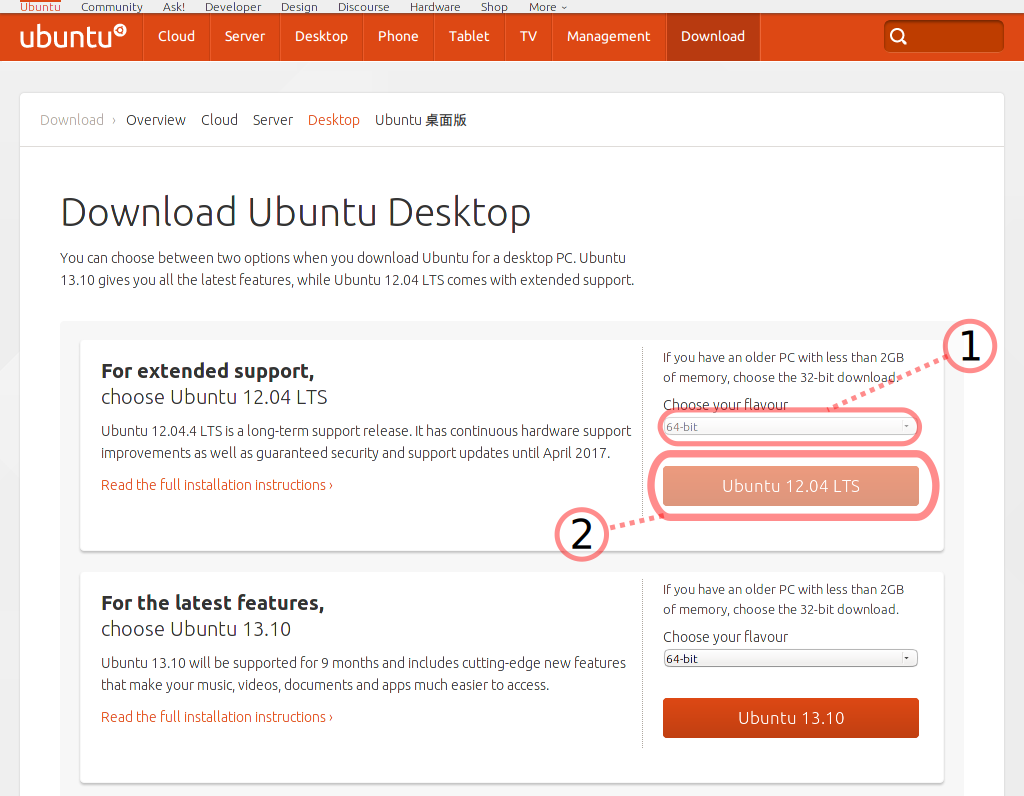
\includegraphics[scale=0.45]{images/instalacja_pobieranie_obrazu.png}
\end{wrapfigure}
Pierwszym etapem instalacji systemu jest pobranie instalatora. W tym celu udaj się na stronę \href{http://www.ubuntu.com/download/desktop}{ubuntu.com} i z górnego paska wybież \textcolor{ubuntu_orange}{Download} a następnie \textcolor{ubuntu_orange}{Desktop}
\begin{description}
\item[(1) Wybór wersji systemu]To pole pozwali ci wybrać pomiędzy 32 a 64 bitową wersją systemu. Domyślnie wybrana jest opcja 64 bitowa. 
\item[(2)]Kliknij na ten przycisk aby przejśc do kolejnego ekranu.
\end{description}
Na kolejnym ekranie będziesz mieć możliwość przekazania dotacji na rzecz Ubuntu. W tym momencie nas to nie interesuje. Przesuń stronę w dół i kliknij na \textcolor{ubuntu_orange}{Not now, take me to the download}. Zostaniesz przeniesiony na kolejną stronę, pobieranie obrazu systemu rozpocznie się za kilka sekund.

Jeżeli twój komputer został wyprodukowany nie dawnej niż 5 lat temu, wersja 64 bitowa będzie na pewno odpowiednia. Jeżeli masz mniej niż 2 gigabajty RAMu, wybierz wersję 32 bitową. Niezależnie jaką wersję wybierzesz, bedziesz mieć dostęp do takiego samego zestawu oprogramowania. Wersja 64 bitowa jest lepiej dopasowana do nowoczesnych systemów. Jeżeli masz jakiekolwiek wątpliwości to wybierz wersję 32 bitową. Taka wersja systemu będzie działać także na 64 bitowym komputerze. Po prostu nie będzie wykorzystywać wszystkich jego możliwości.\\
Jeżeli twoja płyta główna kontrolowana jest przez UEFI, to musisz wybrać system 64 bitowy.

Linki do pobierania bezpośredniego:
\begin{itemize}
\item \href{http://www.ubuntu.com/start-download?distro=desktop&bits=64&release=lts}{Wersja 64 bitowa (733 megabajtów).}
\item \href{http://www.ubuntu.com/start-download?distro=desktop&bits=32&release=lts}{Wersja 32 bitowa (731 megabajtów).}
\end{itemize}
\clearpage

	\subsection{Nagrywanie pobranego obrazu}
		Po zakończeniu pobierania obrazu instalatora należy nagrać go na zewnętrzny nośnik i uruchomić komputer z tego nośnika. Najlepszym rozwiązaniem jest użycie klucza USB (pendrive'a), gdyż obrazy instalacyjne Ubuntu są zbyt duże aby zmieścić się na typowych krążkach CD o pojemności 650 MB. Weź jednak pod uwagę, że nie wszystkie komputery potrafią startować z klucza USB. Jeżeli twój komputer nie pozwala na wykonanie takiej operacji, będziesz musiał użyć płyty DVD lub karty (micro)SD.
\subsubsection{System Windows, nagrywanie na pendriva}
\begin{wrapfigure}{r}{0.5\textwidth}
                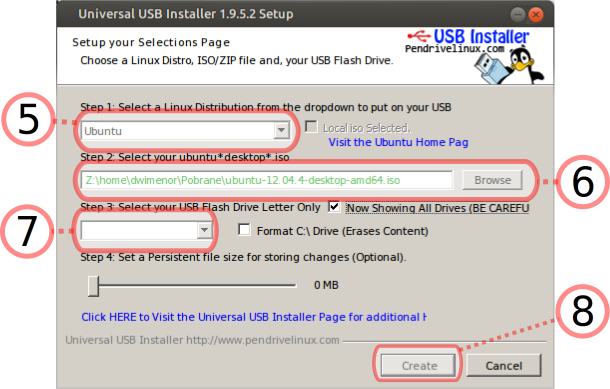
\includegraphics[width=\linewidth]{images/instalacja_nagrywanie_obrazu.png}
\end{wrapfigure}
\noindent Jeżeli chcesz użyć pendrive'a jako nośnika instalacyjnego, upewnij się, żema on przynajmniej 1 GB pojemności (w przeciwnym wypadku instalator się tam po prostu nie zmieści). Jeżeli masz już przygotowany pendrive, wykonaj po kolei następujące kroki:
\begin{enumerate}
\item Pobierz program \href{http://www.pendrivelinux.com/downloads/Universal-USB-Installer/Universal-USB-Installer-1.9.5.2.exe}{Universal USB Installer}.
\item Uruchom pobrany plik.
\item Zaakceptuj umowę licencyjną.
\item Podłącz do komputera pendrive, który ma użyty jako nośnik.
\item Z tej listy wybierz Ubuntu.
\item Kliknij na przycisk “Browse” i wskaż pobrany wcześniej obraz instalatora Ubuntu.
\item Z tej listy wybierz podłączonego wcześniej pendrive'a.\\
\textbf{UWAGA: Wszystkie dane na nim zostaną skasowane!}
\item Kliknij przycisk “CREATE”.
\item Poczekaj na zakończenie operacji.
\end{enumerate}
\clearpage
\subsubsection{System Windows 7 / 8, nagrywanie na płytę DVD}
%TODO zweryfikować, czy Windows 8 też to ma
\begin{wrapfigure}{r}{0.5\textwidth}
                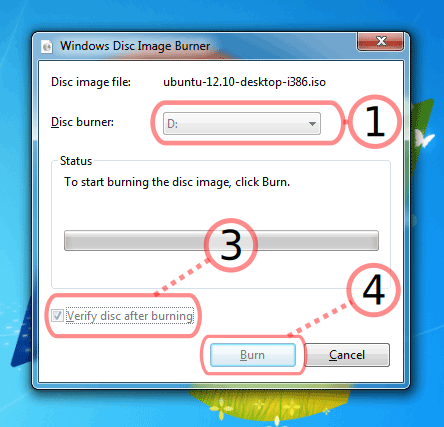
\includegraphics[width=\linewidth]{images/instalacja_nagrywanie_obrazu_DVD.png}
\end{wrapfigure}
Systemy operacyjne Windows 7 i 8 mają wbudowane narzędzie do wypalania plików .iso na płytach. Kliknij prawym przyciskiem myszy na pobrany obraz instalatora Ubuntu, wybierz opcję "Otwórz w" a następnie "Windows Disc Image Burner".
%TODO jak to się po polsku nazywa?
\begin{enumerate}
\item Z tej listy wybierz swoją nagrywarkę.
\item Włóż do wybranego napędu czystą płytę DVD.
\item Upewnij się, że zaznaczone jest pole ”Zweryfikuj dysk po nagraniu”
\item Kliknij na przycisk “Nagraj”.
\end{enumerate}
\clearpage
\subsubsection{System Windows XP i inne starsze wersje, nagrywanie na płytę DVD}
\begin{wrapfigure}{R}{0.5\linewidth}
                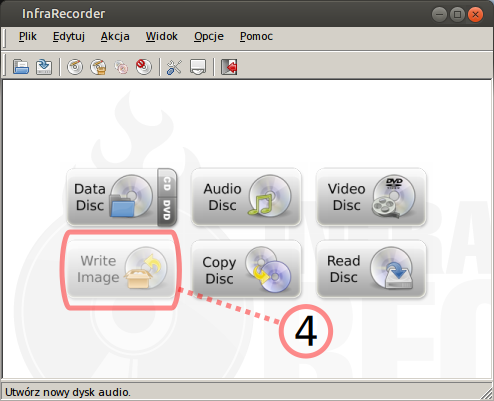
\includegraphics[width=\linewidth]{images/instalacja_nagrywanie_obrazu_DVD_winXP.png}
\end{wrapfigure}
Starsze wersje systemu Windows nie mają wbudowanej możliwości nagrywania płyt DVD. Potrzebne będzie do tego osobne narzędzie służące do wypalania płyt. Obsługa tych programów jest bardzo podobna: należy wybrać opcję Nagrywanie obrazu na płytę. Koniecznie nagrywaj z wykorzystaniem tej opcji, gdyż inne (np. Nagrywanie płyty z danymi lub Tworzenie kopi zapasowej) utworzy dysk, którego twój komputer nie będzie potem wstanie uruchomić. Dla przykładu posłużymy się programem Infra Recorder.
\begin{enumerate}
\item Pobierz i zainstaluj program \href{http://infrarecorder.org/?page_id=5}{Infra Recorder}.
\item Uruchom zainstalowany przed momentem program.
\item Włóż czystą płytę DVD do nagrywarki.
\item W programie Infra Recorder wybierz opcję \textbf{Write Image}.
\item Wybierz pobrany wcześniej obraz instalatora Ubuntu.
\item Kliknij na przycisk \textbf{OK}.
\end{enumerate}
\clearpage

		\subsubsection{System Linux, nagrywanie na pendriva}
\begin{wrapfigure}{r}{0.5\textwidth}
		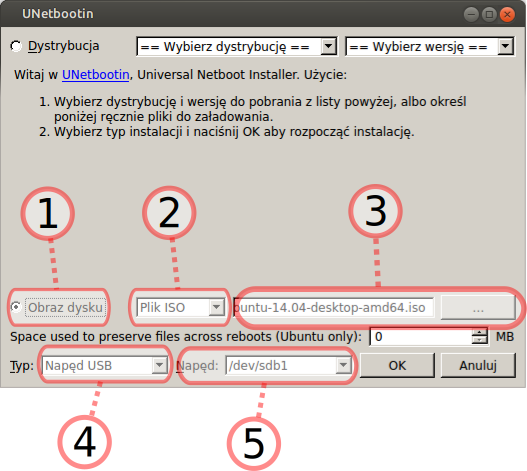
\includegraphics[width=\linewidth]{images/instalacja_nagrywanie_obrazu_linux.png}
\end{wrapfigure}
W systemach operacyjnych Linux do nagrywania obrazu na pendriva najlepiej posłużyć się programem UnetBootin, dostępnym w każdej dystrybucji. Podłącz do komputera napęd USB, który chcesz przeznaczyć na instalator Ubuntu.
\begin{enumerate}
\item Zaznacz pole Obraz dysku
\item Z menu wybierz Plik ISO
\item W to pole podaj ścierzkę do pobranego wcześniej obrazu instalatora Ubuntu. Wciśnij przycisk oznaczony trzema kropkami (\ldots) i wskaż plik.
\item W tym menu wybierz Napęd USB
\item Z tego menu wybierz podłączonego wcześniej pendriva.\\
\textbf{UWAGA: Wszystkie dane na nim zostaną skasowane!}
\item Kliknij przycisk OK aby rozpoczać nagrywanie
\end{enumerate}
\clearpage
\subsubsection{System Linux, nagrywanie na DVD}
%TODO potrzebny obrazek z włożoną płytą DVD i wybranym obrazem ubuntu 14.04
\begin{wrapfigure}{L}{0.5\textwidth}
		\includegraphics[width=\linewidth]{images/instalacja_nagrywanie_obrazu_linux_DVD.png}
\end{wrapfigure}
Aby nagrać obraz na płytę DVD potrzebujesz odpowiedniego programu. W tym przykładzie posłużymy się dostępną w większości dystrybucji nagrywarką Brasero. Kliknij prawym przyciskiem myszy na pobrany wcześniej obraz instalatora Ubuntu, wybierz Otwórz w a następnie Brasero. W otwartym oknie zostaniesz poproszony o włożenie czystej płyty DVD. Zrób to, a nastepnie kliknij na przycisk Nagraj.
\clearpage
	\subsection{Przygotowanie do instalacji}
		\label{sec:przygotowanie_windows}Powinieneś mieć świadomość, że instalacja innego systemu operacyjnego na dysku twardym twojego komputera zawsze wiąże się z ryzykiem utraty danych. Niestety, czasem zdarzają się nieprzewidziane sytuacje. Zanik zasilania w czasie partycjonowania dysku twardego najczęściej prowadzi do utraty jego zawartości. Do rzadkości nie należy również sytuacja, w której ktoś przez zwykłą nieuwagę  nadpisze jeden system drugim i w ten sposób utraci dane. Zanim przystąpisz więc do instalacji systemu Ubuntu, upewnij się, że wszystkie ważne dane zostały zabezpieczone na zewnętrznych nośnikach. Innymi słowy~---~zrób kopię zapasową.

\subsubsection{Przygotowanie do instalacji --- Windows --- wskazówki ogólne}
Warto też wyeksportować dane z programów takich jak przeglądarka internetowa (zakładki), klient pocztowy(konta, kalendarze i kontakty), czy też komunikator internetowy (konta, historia rozmów, znajomi). Nie zapomnij zrobić kopii zapasowej dokumentów oraz swojej kolekcji muzyki. Jeżeli zainstalujesz Ubuntu obok Windowsa, będziesz mieć dostęp do swoich plików. Niestety, w drugą stronę to już nie działa --- na systemach Windows nie ma możliwości podglądu plików znajdujących na partycjach Ubuntu\footnote{To jest możliwe, ale dosyć skomplikowane i wykracza poza zakres tego przewodnika.}.
Ważnym krokiem jest ustalenie, czy twoja płyta główna zarządzana jest przez UEFI (a jeżeli tak, to jakie opcje są włączone).

W konsoli systemu Windows\footnote{\menu{Start>Uruchom} wpisz ,,cmd'' i wciśnij \keys{\returnwin}.} wpisz \textcolor{ubuntu_orange}{Confirm-SecureBootUEFI}. System może zwrócić jedną z trzech informacji:
\begin{itemize}
\item \textcolor{ubuntu_orange}{Cmdlet not supported on this platform} --- Ten komputer nie korzysta z SecureBoot. Nie potrzebujesz podejmować żadnych dodatkowych kroków, wystarczy włożyć przygotowany nośnik instalacyjny i zainstalować Ubuntu.
\item \textcolor{ubuntu_orange}{Nazwa ,,Confirm-SecureBootUEFI'' nie jest rozpoznawana jako polecenie wewnętrzne lub \linebreak zewnętrzne, plik wykonywalny lub plik wsadowy} --- Ten komputer nie korzysta z SecureBoot. Nie potrzebujesz podejmować żadnych dodatkowych kroków, wystarczy włożyć przygotowany nośnik instalacyjny i zainstalować Ubuntu.
\item \textcolor{ubuntu_orange}{False} --- Ten komputer ma UEFI, ale nie korzysta z SecureBoot. Przejdź do sekcji \ref{sec:przygotowanie_windows8} Przygotowanie do instalacji --- Windows 8.
\item \textcolor{ubuntu_orange}{True} --- Ten komputer ma UEFI i korzysta z SecureBoot. Przejdź do sekcji \ref{sec:przygotowanie_windows8} Przygotowanie do instalacji --- Windows 8.
\end{itemize}
\subsubsection{Przygotowanie do instalacji --- Windows 8}
\label{sec:przygotowanie_windows8}
Windows 8 wymusił na producentach sprzętu stosowanie technologi UEFI (zamiast BIOS-u) oraz SecureBoot (zabezpieczenie komputera przed zmianami systemu operacyjnego), co znacznie utrudniło instalację innych systemów operacyjnych. Ubuntu jest przygotowane do współpracy z Windows 8, ale Windows nie jest przygotowany do współdzielenia komputera z innymi systemami operacyjnymi. Pamiętaj, że jeżeli posiadasz UEFI (a używanie Windows 8 na to wskazuje), to potrzebujesz Ubuntu w wersji 64-bitowej. Systemy 32-bitowe nie są obsługiwane przez technologię UEFI\footnote{A przynajmniej nie bez dużej ilości kombinowania.}.

W tym momencie warto przygotować wolną przestrzeń na dysku dla systemu Ubuntu. Ten punkt można wykonać zarówno teraz, jak i podczas instalacji Ubuntu --- jeżeli jednak używasz Windows 8, lepiej zrobić to teraz. Wciśnij kombinację klawiszy \keys{Super + r} i uruchom program \textcolor{ubuntu_orange}{compmgmt.msc}. W~uruchomionym programie utwórz partycję dla Ubuntu. Absolutne minimum w przypadku tej partycji to 6,2 gigabajta. Ubuntu potrzebuje około 4 GB na podstawową instalację, pozostałe miejsce będzie można przeznaczyć na instalację oprogramowania oraz pliki użytkownika. Jak wspomniano powyżej, 6,2 gigabajta to naprawdę minimum --- tak naprawdę zalecamy stworzenie partycji liczącej sobie przynajmniej 20 GB.

Windows 8 korzysta z opcji ,,Szybkiego uruchamiania'' (\textit{Fast Boot}), która uniemożliwia Ubuntu dostęp do plików znajdujących się na partycji Windows. Jedynym sposobem na obejście tego problemu jest wyłączenie ,,Szybkiego uruchamiania''. Otwórz \menu{{Panel Sterowania}>{Opcje Zasilania}}, a następnie odznacz \textcolor{ubuntu_orange}{Włącz szybkie uruchamianie}.
\subsubsection{Przygotowanie do instalacji --- Linux}
\label{sec:przygotowanie_linux}
Instalacja kilku systemów Linux obok siebie nie powoduje żadnych problemów, powinieneś jednak wiedzieć o paru sprawach. W systemach operacyjnych należących do tej rodziny pliki użytkownika przechowywane są w katalogu /home. Dobrą praktyką jest wydzielenie osobnej partycji na ten katalog, aby przy reinstalacji systemu nie tracić swoich ustawień.

Jeżeli instalujesz jednego Linuksa obok drugiego, pomysł wykorzystania jednej partycji domowej dla obu systemów może wyglądać naprawdę kusząco. To jest możliwe, ale weź pod uwagę, że każdy z~tych systemów może korzystać z innych plików --- może się więc okazać, że nie wszystkie ustawienia będą prawidłowo odczytywane w obu dystrybucjach (szczególnie jeżeli używasz różnych środowisk graficznych). Przy takiej konfiguracji ważne jest też, aby nazwa użytkownika oraz jego grupy były takie same na obu systemach. Jeżeli instalowane obok siebie dystrybucje Linuksa dzieli wiele różnic, lepiej nie korzystać ze wspólnego katalogu domowego, a zamiast tego umieścić dokumenty, filmy, czy muzykę w miejscu dostępnym dla obydwu systemów.

Jeszcze jedna uwaga --- niezależnie od tego, ile dystrybucji Linuksa planujesz zainstalować, wystarczy im jedna, wspólna partycja wymiany (swap).

	\subsection{Uruchomienie instalatora}
		\subsubsection{Ponowne uruchomienie komputera}
Jeżeli dysponujesz już  nośnikiem instalacyjnym, nie pozostaje nic innego, jak uruchomić instalator i zainstalować system na dysku twardym komputera. Jeśli korzystasz z tego przewodnika w trybie online, dobrym pomysłem będzie wydrukowanie kilku kolejnych stron. Może się zdarzyć, że w czasie instalacji stracisz dostęp do internetu i zostaniesz tym samym odcięty od zawartych tutaj informacji.
Przed przystąpieniem do instalacji koniecznie zapoznaj się także z następującymi sekcjami:
\begin{itemize}
\item \ref{sec:przygotowanie_windows} \textcolor{ubuntu_orange}{Przygotowanie do instalacji - Windows - wskazówki ogólne}: ta sekcja zawiera przydatne informacje dla osób migrujących z systemów Windows.
\item \ref{sec:przygotowanie_windows8} \textcolor{ubuntu_orange}{Przygotowanie do instalacji - Windows 8}: specyficzne porady dla systemu Windows 8. Koniecznie ten fragment przewodnika, jeżeli instalujesz Ubuntu obok Windows 8 lub próbujesz zainstalować Ubuntu zamiast Windows 8.
%TODO http://askubuntu.com/questions/221835/installing-ubuntu-on-a-pre-installed-windows-8-64-bit-system-uefi-supported
\item \ref{sec:przygotowanie_linux} \textcolor{ubuntu_orange}{Przygotowanie do instalacji - Linux}: ogólne wskazówki dla osób instalujących Ubuntu obok innych dystrybucji Linuksa.
\end{itemize}

Zrestartuj swój komputer i uruchom go z przygotowanego nośnika instalacyjnego. W większości przypadków wiąże się to z ręcznym wskazaniem odpowiedniego napędu podczas uruchamiania komputera. Jeśli twój komputer wyposażony jest w system UEFI, cała ta procedura będzie znacznie bardziej skomplikowana.
\subsubsection{Zmiana kolejności bootowania}
Kiedy rozpocznie się rozruch komputera, jeszcze przed załadowaniem się systemu operacyjnego musisz poinformować maszynę, że tym razem  zamiast systemu zainstalowanego na twardym dysku ma ona wykorzystać przygotowany przez nas instalator. Każdy producent płyt głównych podchodzi do tej kwestii w nieco odmienny sposób, jednak najczęściej procedura będzie się pokrywać z jednym z opisanych poniżej scenariuszy:
\begin{itemize}
\item Niektóre komputery podczas rozruchu pokazują napis \textcolor{ubuntu_orange}{Press F12 to select boot device}. Kluczowymi słowami są tutaj \textcolor{ubuntu_orange}{Boot Device}, \textcolor{ubuntu_orange}{Boot order} lub podobne . Wciśnij wskazany klawisz (w tym konkretnym przypadku \keys{F12}, ale nie jest to regułą) i z wyświetlonego menu wybierz nośnik instalacyjny. Niektóre komputery wykrywają pendrive'y jako dyski twarde i musisz wskazać właśnie taki dysk twardy a nie port USB. Jeżeli na liście nie ma naszego instalatora, zresetuj komputer i spróbuj ponownie.
\item Jeżeli zobaczysz napis \textcolor{ubuntu_orange}{Press ESC to enter setup} lub coś podobnego, twoim słowem kluczowym będzie \textcolor{ubuntu_orange}{Setup}. Wciśnięcie odpowiedniego klawisza (\keys{\escwin}, \keys{\delwin} lub któryś z klawiszy funkcyjnych) spowoduje uruchomienie programu konfiguracyjnego płyty głównej. W tym programie przejdź do sekcji \menu{{Advanced BIOS Features}>{First Boot Device}}. Wskaż napęd CD-ROM lub napęd USB (względnie drugi dysk twardy, jeżeli pendrive jest rozpoznawany jako dysk twardy). Wróć do menu głównego (klawisz \keys{\escwin} cofa o jedno menu) i zapisz zmiany (najczęściej \keys{F10}, czasem \keys{\escwin} i potwierdzenie przy pomocy klawisza \keys{y}). W tym momencie komputer samoczynnie się zrestartuje.
\end{itemize}
\subsubsection{Uruchomienie instalatora UEFI}
Po wybraniu urządzenia z nośnikiem instalacyjnym komputer rozpocznie proces jego uruchamiania. Może to potrwać od kilku do kilkunastu sekund. W tym czasie ekran komputera będzie czarny bądź będą się przez niego przewijały napisy.\\
Jeżeli twoja maszyna pracuje pod kontrolą UEFI, to pierwszy ekran instalatora będzie wyglądał jak na poniższym rysunku:
\begin{center}
        \includegraphics[width=\linewidth]{images/instalacja_UEFI_boot.png}
\end{center}

\noindent Do wyboru masz następujące opcje:
\begin{itemize}
\item \textcolor{ubuntu_orange}{Try Ubuntu without installing (Wypróbuj Ubuntu bez instalowania)} - Uruchomi system Ubuntu bez instalacji go na dysku twardym. W ten sposób możesz przetestować Ubuntu i zobaczyć jak działa w praktyce. Wszystkie zmiany jakie wprowadzisz w systemie zostaną odrzucone po wyłączeniu komputera. Należy pamiętać, że w tym trybie Ubuntu działa bardzo wolno, gdyż musi korzystać z powolnego nośnika (płyta DVD lub pendriv). Po normalniej instalacji Ubuntu będzie działać z pełną wydajnością. Skrót do instalatora systemu znajduje się na Pulpicie.
\item \textcolor{ubuntu_orange}{Install Ubuntu (Zainstaluj Ubuntu)} - Ta opcja bezpośrednio uruchomi instalator Ubuntu bez wczytywania całego systemu.
\item \textcolor{ubuntu_orange}{OEM Install (Instalacja dla producentów sprzętu} - Ta opcja pozwala zainstalować podstawowy system bez tworzenia użytkownika. Przy pierwszym uruchomieniu zostaniesz poproszony o stworzenie nowego użytkownika.
\item \textcolor{ubuntu_orange}{Check disk for defects (Sprawdź płytę pod kontem błędów odczytu} - Ta opcja sprawdzi czy używany nośnik został prawidłowo utworzony.\\
Przed przystąpieniem do instalacji systemu warto wykonać sprawdzenie nośnika instalacyjnego. Potrwa to góra kilka minut a pozwoli zaoszczędzić czas w przyszłości. Podczas przeprowadzania testów komputer może wyświetlać tylko czarny ekran. Jeżeli nie znajdzie żadnych błędów, otrzymasz komunikat \textcolor{ubuntu_orange}{Check Finished: No errors found. Press any key to reboot your system (Zakończono sprawdzanie: Nie znaleziono błędów. Wciśnij dowolny klawisz aby zresetować komputer)}. Po ponownym uruchomieniu komputera możesz przystąpić do instalacji. Jeżeli znaleziono jakiekolwiek błędy to należy ponownie przygotować nośnik instalacyjny. Użycie wadliwego instalatora doprowadzi do uszkodzenia systemu. 
\end{itemize}
\clearpage
\subsubsection{Uruchomienie instalatora BIOS}
\label{instalacja_uruchomienie}
\begin{wrapfigure}{l}{0.5\textwidth}
                \includegraphics[width=\linewidth]{images/instalacja_BIOS_boot.png}
\end{wrapfigure}

Po wybraniu urządzenia z nośnikiem instalacyjnym komputer rozpocznie proces jego uruchamiania. Może to potrwać od kilku do kilkunastu sekund. W tym czasie ekran komputera będzie czarny bądź będą się przez niego przewijały napisy. Kiedy ekran komputera zmieni kolor z czarnego na fioletowy wciśnij dowolny klawisz aby wejść do ustawień instalatora. Jeżeli tego nie zrobisz, instalator usruchomi się w trybie \textcolor{ubuntu_orange}{Wypróbuj Ubuntu bez Instalacji}.

Na początek wybierz język w jakim system będzie się z tobą komunikował. Przy pomocy klawiszy kursora przejdź do trzeciej kolumny. Język Polski znajduje się mniej więcej w połowie tej kolumny. Wciśnij \keys{returnwin} aby zatwierdzić.

\begin{itemize}
\item \textcolor{ubuntu_orange}{Wypróbuj Ubuntu bez instalowania} - Uruchomi system Ubuntu bez instalacji go na dysku twardym. W ten sposób możesz przetestować Ubuntu i zobaczyć jak działa w praktyce. Wszystkie zmiany jakie wprowadzisz w systemie zostaną odrzucone po wyłączeniu komputera. Należy pamiętać, że w tym trybie Ubuntu działa bardzo wolno, gdyż musi korzystać z powolnego nośnika (płyta DVD lub pendriva). Po normalniej instalacji Ubuntu będzie działać z pełną wydajnością. Skrót do instalatora systemu znajduje się na Pulpicie.
\item \textcolor{ubuntu_orange}{Zainstaluj Ubuntu} - Ta opcja bezpośrednio uruchomi instalator Ubuntu bez wczytywania całego systemu.
\item \textcolor{ubuntu_orange}{Sprawdź płytę pod kontem błędów odczytu} - Ta opcja sprawdzi czy używany nośnik został prawidłowo utworzony.\\
Przed przystąpieniem do instalacji systemu warto wykonać sprawdzenie nośnika instalacyjnego. Potrwa to góra kilka minut a pozwoli zaoszczędzić czas w przyszłości. Podczas przeprowadzania testów komputer może wyświetlać tylko czarny ekran. Jeżeli nie znajdzie żadnych błędów, otrzymasz komunikat "Check Finished: No errors found. Press any key to reboot your system" (Zakończono sprawdzanie: Nie znaleziono błędów. Wciśnij dowolny klawisz aby zresetować komputer). Po ponownym uruchomieniu komputera możesz przystąpić do instalacji. Jeżeli znaleziono jakiekolwiek błędy to należy ponownie przygotować nośnik instalacyjny. Użycie wadliwego instalatora doprowadzi do uszkodzenia systemu. 
\item \textcolor{ubuntu_orange}{Sprawdź pamięć} - Ta opcja uruchomi program memtest, który wykona test pamięci operacyjnej komputera (RAM). Uszkodzona pamięć jest jedną z częstszych przyczyn błędów instalatora jak i wpływa negatywnie na pracę zainstalowanego systemu.
\item \textcolor{ubuntu_orange}{Uruchom system z pierwszego dysku twardego} - Ta opcja kończy pracę instalatora i uruchamia podstawowy system operacyjny komputera.
\end{itemize}

Dodatkowe opcje widoczne na dolnym pasku uruchamia się wciskając odpowiedni klawisz funkcyjny:
\begin{itemize}
\item \keys{F1} - Wyświetla pomoc, wraz z szczegółowym opisem poszczególnych opcji konfiguracyjnych.
\item \keys{F2} - Zmiana języka instalatora.
\item \keys{F3} - Zmiana układu klawiatury.
\item \keys{F4} - Zmiana trybu pracy instalatora:
        \begin{description}
        \item[\textcolor{ubuntu_orange}{Zwykły}] - Tryb podstawowy, teraz się w nim znajdujesz
        \item[\textcolor{ubuntu_orange}{Użycie nośnika aktualizującego sterowniki}] - ?? %TODO o co biega?
        \item[\textcolor{ubuntu_orange}{Instalacja OEM (dla producentów sprzętu)}] - Ta opcja pozwala zainstalować podstawowy system bez tworzenia użytkownika. Przy pierwszym uruchomieniu zostaniesz poproszony o stworzenie nowego użytkownika.
        \end{description}
\item \keys{F5} - Pozwala włączyć/wyłączyć dodatkowe opcje ułatwiające instalacje osobom niepełnosprawny (Klawiatura ekranowa, lupa, wysoki kontrast, czytnik ekranu, klawiatura Braille'a)
\item \keys{F6} - Dodatkowe parametry rozruchu, pomocne w przypadku napotkania problemów ze sprzętem.
\end{itemize}
\clearpage

	\subsection{Graficzny instalator Ubuntu}
		Niezależnie od tego czy posiadasz płytę główną z BIOSem czy z UEFI, w poprzednim punkcie powinieneś wybrać "Zainstaluj Ubuntu". Ta metoda jest szybsza od "Wypróbuj Ubuntu bez instalowania" gdyż nie wymaga załadowania całego systemu. Jeżeli mimo wszystko uruchomiłeś cały system, to na jego pulpicie znajdziesz ikonę "Zainstaluj Ubuntu" (lub "Install Ubuntu", jeżeli nie zmienięłś języka). Od tego momentu instalacja przebiega w identyczny sposób.
\subsubsection{Wybór języka}
Pierwszy ekran instalatora pozwala wybrać język. Jeżeli wcześniej nie zmieniłeś języka na Polski to teraz masz ku temu okazję. Język wybrany podczas instalacji będzie także domyślnym językiem zainstalowanym w systemie.
\subsubsection{Sprawdzenie kompatybilności sprzętu, wybór dodatkowych komponentów}
Na tym etapie instalator sprawdzi, czy na dysku twardym jest wystarczająco miejsca aby zainstalować Ubuntu. Połączenie z internetem nie jest wymagane aby zainstalować system. Połączenie z internetem jest niezbędne aby zainstalować spolszczenie systemu, aktualizacje oraz dodatkowe wtyczki.
\begin{description}
\item[Pobieranie aktualizacji podczas instalacji] - Instalator pobierze i zainstaluje wszystkie aktualizacje, które zostały wydane od dnia premiery systemu.
\item[Instalacja licencjonowanego oprogramowania] - Instalator pobierze i zainstaluje kodeki audio/video oraz plugin flash do przeglądarki internetowej. Jeżeli posiadasz kartę graficzną firm Nvidia lub AMD to zostaną też zainstalowane dodatkowe sterowniki dostarczane przez tych producentów.
\end{description}
\subsubsection{Partycjonowanie dysku twardego}
Jest to najważniejszy etap instalacji. W tym miejscu można dokonać cudów jak i zniszczyć cały dysk twardy. Jako, że prawidłowe partycjonowanie dysku twardego to bardzo szeroki temat to poświęciliśmy mu cały osobny rozdział. Kiedy go przeczytasz i podzielisz swój dysk twardy, wróć do tego miejsca.
\subsubsection{Wybór strefy czasowej}
Na tym etapie należy wybrać lokalizację tego komputera, tak aby system mógł wyświetlać prawidłowy czas i automatycznie dostosowywać się do zmian pomiędzy czasem letnim i zimowym. Jeżeli w trakcie instalacji masz połączenie z internetem to odpowiednia lokalzacja zostanie sama wybrana. Jeżeli nie masz dostępu do internetu w pole wpisz "Warsaw". Stolica naszego kraju okresla też nasza strefę czasową.
\subsubsection{Wybór ukłądu klawiatury}
Ten ekran pozwala wybrać układ klawiatury. Jeżeli wybrałeś wcześniej język Polski, to standardowa polska klawiatura zostanie tutaj automatycznie wybrana. W polu możesz wpisać kilka znaków aby sprawdzić czy zaznaczony układ odpowiada rzeczywistości. Pierwsza opcja ("Polski") to standardowa klawiatura 101 klawiszy, zwana potocznie ukłądem programisty.
\subsubsection{Dane użytkownika}
To już ostatni etap instalacji. Te pola należy uzupełnić aby system mógł cię prawidłowo zidentyfikować.
\begin{description}
\item[Imię i nazwisko użytkownika] - Pole nieobowiązkowe, ale jeżeli uzupełnisz te dane to system będzie się do ciebie zwracał z imienia i nazwiska zamiast używać loginu (np. Jan Kowalski).
\item[Nazwa komputera] - Określa jak będzie się nazywał twój komputer (np. laptop).
\item[Nazwa użytkownika] - Twój login do systemu (np. jan\_kowalski albo twój pseudonim). Login nie może zawierać dużych liter, spacji ani znaków specjalnych.
\item[Hasło] - Hasło do komputera. Hasło zabezpiecza system przed nieuprawnionym dostępem. Uwaga: Ustawienie hasła uniemożliwia innym zalogowanie się do twojego konta, jednak nie zabezpiecza innych przed podglądem twoich dany o ile ich nie zaszyfrujesz. 
\item[Potwierdzenie hasła] - Wpisz ponownie to samo hasło co w polu powyżej.
\item[Automatyczne logowanie] - Jeżeli zaznaczysz to pole, to system automatycznie zaloguje tego użytkownika po uruchomieniu. Nie będzie potrzebne podawanie hasła aby uzyskać dostęp do komputera.
\item[Wymaganie hasła do zalogowania] - Po uruchomieniu komputera będziesz musiał podać hasło aby uzyskać dostęp do swojego konta.
\item[Szyfrowanie dysku twardego] - Jeżeli zaznaczysz tą opcję to zawartość dysku twardego zostanie zaszyfrowana. Nikt nie znający hasła nie będzie mógł uzyskać dostępu do twoich plików. Jeżeli zapomnisz hasła to równie dobrze możesz sformatować dysk twardy i zainstalować system na nowo.
\end{description}
\subsubsection{Instalacja}
Teraz system dokona instalacji na dysku twardym i ewentualnie pobierze i zainstaluje paczki językowe, aktualizacje i dodatkowe oprogramowanie. Proces ten może potrwać od kilku do kilkunastu minut w zależności od klasy komputera, ilości zadań do wykonania oraz szybkości łącza internetowego.
	\subsection{Partycjonowanie dysku twardego}
		\label{subsec:partycjonowanie}
Partycjonowanie to proces zmiany układu partycji na dysku twardym. Jest to najważniejszy etap instalacji systemu gdyż to od niego w dużej mierze zależy jak system będzie działał. Pamiętaj, że na tym etapie pracujesz na danych zapisanych na dysku twardym. Chwila nieuwagi może spowodować utratę jego zawartości.
\subsubsection{Ile miejsca przeznaczyć na Ubuntu}
\label{ile_miejsca}
Wirtualny dysk twardy użyty w tym przewodniku ma tylko 26.8 gigabajta pojemności. Twój dysk twardy będzie miał zapewne kilkaset gigabajtów (jeżeli nie kilka terabajtów) pojemności. Dlatego też liczby jakimi się tu posługujemy będą miały niewielkie przełożenie na sytuację na twoim komputerze. W tym miejscu powinieneś się jednak zastanowić ile miejscach chcesz przeznaczyć na Ubuntu.
Ogólnie rzecz ujmując sprawa wygląda następująco
\begin{itemize}
\item \textcolor{ubuntu_orange}{Partycja główna, root, /} - 6,2 Gigabajta to absolutne minimum. 10 gigabajtów da pewną elastyczność i pozwoli zainstalować więcej programów. Nie ma potrzeby przesadzać w drugą stronę i tworzyć zbyt dużej partycji głównej, gdyż wolna przestrzeń będzie niewykorzystana. 15-20 gigabajtów w zupełności wystarczy.
\item \textcolor{ubuntu_orange}{Partycja wymiany, swap} - na tej partycji zapisywane są dane, które nie mieszczą się w pamięci operacyjnej. Tutaj też przechowywany jest obraz RAMu kiedy poddajesz komputer hibernacji. Jeżeli korzystasz z hibernacji to wielkość partycji swap powinna być co najmniej taka jak ilość pamięci operacyjnej twojego komputera. Jeżeli nie planujesz korzystać z hibernacji to możesz nie tworzyć partycji wymiany. Jednak zaleca się jej stworzenie, jeżeli masz mniej niż 2 gigabajty RAMu. W takim wypadku nawet jeżeli nie korzystasz z hibernacji to dobrze jest stworzyć niewielką (300 - 400 megabajtów) partycję swap.
\item \textcolor{ubuntu_orange}{Partycja domowa, /home} - W katalogu /home przechowywane są prywatne pliki użytkownika: zawartość pulpitu, dokumenty, filmy, muzyka i ustawienia programów. Katalog domowy może znajdować się na głównej partycji (/, root) lub można go wydzieć. Dobrą praktyką jest wydzielenie takiej partycji, gdyż w razie reinstalacji systemu nie trzeba będzie jej kasować. Nadpisana pozostanie tylko partycja główna, zaś wszystkie prywatne dane pozostaną niezmienione. Wielkość tej partycji zależy tylko i wyłącznie od tego jak wiele miejsca chcesz na nią przeznaczyć i jak wiele rzeczy zamierzasz na niej trzymać. 
\end{itemize}
\clearpage
\subsubsection{Czysty dysk - wykorzystanie całego dostępnego miejsca}
\begin{center}
        \includegraphics[width=\linewidth]{images/instalator_partycjonowanie_proste.png}
\end{center}

Jeżeli na dysku twardym nie ma żadnego innego systemu operacyjnego, instalator Ubuntu zaproponuje wykorzystanie całej dostępnej przestrzeni. Instalator sam dobierze odpowiedni rozmiar partycji systemowej, partycji wymiany oraz partycji użytkownika.
\begin{flushright}
Kliknij na przycisk \textcolor{ubuntu_orange}{Zainstaluj} aby przejść dalej.\\
Zostaniesz poproszony o potwierdzenie. Upewnij się, że wszystko jest w porządku i kliknij \textcolor{ubuntu_orange}{Naprzód}.\\
W tym momencie wybrane zmiany zostaną zapisane na dysku twardym.
\end{flushright}
\clearpage
\subsubsection{Instalacja obok zainstalowanego Ubuntu}
\begin{center}
        \includegraphics[width=\linewidth]{images/instalator_partycjonowanie_obok_ubuntu.png}
\end{center}

Jeżeli instalator wykryje obecność wcześniej zainstalowanej innej wersji Ubuntu to zaproponuje kilka innych rozwiązań.
Po pierwsze zaproponuje aktualizację zainstalowanego systemu do najnowszego wydania. Wszystkie dane w katalogu domowym użytkownika zostaną zachowane: muzyka, filmy, dokumenty, pliki na pulpicie, osobiste ustawienia programów, zakładki i historia przeglądarki itp.

Skasowane zostaną zainstalowane w systemie programy oraz ustawienia systemowe. Instalator zaktualizuje istniejące na dysku oprogramowanie i ewentualnie pobierze aktualizacje z internetu (jeżeli wybrałeś wcześniej tą opcję).
Drugą opcją jest usunięcie zainstalowanego Ubuntu i ponowna instalacja systemu. Wszystkie dane zostaną wymazane.
\begin{flushright}
Kliknij na przycisk \textcolor{ubuntu_orange}{Zainstaluj} aby przejść dalej.\\
Zostaniesz poproszony o potwierdzenie. Upewnij się, że wszystko jest w porządku i kliknij \textcolor{ubuntu_orange}{Naprzód}.\\
W tym momencie wybrane zmiany zostaną zapisane na dysku twardym.
\end{flushright}
\clearpage
\subsubsection{Instalacja obok Windowsa}
\begin{center}
        \includegraphics[width=\linewidth]{images/instalator_partycjonowanie_obok_wondows7.png}
\end{center}

Jeżeli instalator wykryje obecność wcześniej zainstalowanego systemu Windows to zaproponuje inne rozwiązanie. Opcja "Zamiana Windows na Ubuntu" wymaże całą zawartość partycji Windows (wraz ze wszystkimi danymi) i zamiast tego zainstaluje Ubuntu. Zostało to opisane dwie strony wcześniej.
\begin{flushright}
Kliknij na przycisk \textcolor{ubuntu_orange}{Zainstaluj} aby przejść dalej.
\end{flushright}
\clearpage
\begin{center}
        \includegraphics[width=\linewidth]{images/instalator_partycjonowanie_obok_wondows7_2.png}
\end{center}

Drugą możliwością jest instalacja Ubuntu obok już zainstalowanego systemu Windows. Jeżeli wybierzesz tę opcję to następny ekran pozwoli wybrać o ile instalator ma zmniejszyć partycję na której zainstalowany jest system Windows. Użyj myszy aby przesunąć pomarańczową podziałkę w lewo (więcej miejsca dla Ubuntu) lub w prawo(więcej miejsca dla Windowsa). Oryginalna partycja systemu Windows jest oznaczona na tym obrazie jako "Pliki". Pamiętaj, że Ubuntu potrzebuje minimum 6,2 gigabajta przestrzeni, ale tak mała partycja zostanie prawie w całości wypełniona przez system i na Twoje pliki pozostanie niewiele miejsca.
\begin{flushright}
Kliknij na przycisk \textcolor{ubuntu_orange}{Zainstaluj} aby przejść dalej.\\
Zostaniesz poproszony o potwierdzenie. Upewnij się, że wszystko jest w pożądku i kliknij \textcolor{ubuntu_orange}{Naprzód}.\\
W tym momencie wybrane zmiany zostaną zapisane na dysku twardym.
\end{flushright}
\clearpage
\subsubsection{Szyfrowanie dysku twardego}
\begin{center}
        \includegraphics[width=\linewidth]{images/instalator_partycjonowanie_szyfrowanie1.png}
\end{center}

Przy wyborze jednego z automatycznych rozwiązań partycjonowania miałeś możliwości zastosowania szyfrowania dysku twardego. Wybranie tej opcji ukaże ci okno jak na powyższym obrazku. Zaszyfrowanie dysku twardego sprawie, że nikt nie uzyska dostępu do twoich danych ani nie zmodyfikuje zainstalowanego systemu. Wadą tego rozwiązania jest pewien narzut na procesor komputera i związane z tym zmniejszenie płynności działania komputera. Nowoczesne procesory zapewniają akcelerację sprzętową dla obliczeń kryptograficznych, w związku z czym utrata wydajności będzie się mieścić w granicach 5\% przy intensywnych opracacjach dyskowych.
\begin{flushright}
Kliknij na przycisk \textcolor{ubuntu_orange}{Zainstaluj} aby przejść dalej.
\end{flushright}
\clearpage
\begin{center}
        \includegraphics[width=\linewidth]{images/instalator_partycjonowanie_szyfrowanie2.png}
\end{center}

Na tym ekranie podaj hasło - klucz do dysku twardego. To nie jest to samo hasło, które ustawisz dla swojego systemowego konta a jedynie hasło umożliwiające dostęp do danych zapisanych na dysku twardym. Pamiętaj, że jeżeli zapomnisz hasła jakie zostanie tu wprowadzone, nie będzie możliwości odzyskania zaszyfrowanych danych. Postaraj się też aby hasło nie było łatwe do odgadnięcia, ale łatwe dla ciebie do zapamiętania.

Opcja "Zamazanie pustej przestrzeni dysku" powoduje, że niewykorzystywana, wolna przestrzeń dysku zostanie nadpisana losowymi danymi. Taka operacja znacznie utrudnia potencjalnym włamywaczom włamanie się do twoich danych. Miej na uwadze, że zamazywanie pustej przestrzeni może trwać bardzo długo, w zależności do tego ile miejsca przeznaczysz na Ubuntu.
\begin{flushright}
Kliknij na przycisk \textcolor{ubuntu_orange}{Zainstaluj} aby przejść dalej.\\
Zostaniesz poproszony o potwierdzenie. Upewnij się, że wszystko jest w porządku i kliknij \textcolor{ubuntu_orange}{Naprzód}
W tym momencie wybrane zmiany zostaną zapisane na dysku twardym.\\
\end{flushright}
\clearpage
\subsection{Zaawansowane partycjonowanie}
\begin{center}
        \includegraphics[width=\linewidth]{images/instalator_partycjonowanie_gparted1.png}
\end{center}

\textcolor{ubuntu_orange}{Użycie innego rozwiązania} uruchamia program GParted, który umożliwia nieograniczone modyfikowanie partycji na dysku twardym. Jest to opcja dla bardziej zaawansowanych użytkowników, którzy mają świadomość tego jak działa partycjonowanie i jak powinien zostać podzielony ich dysk twardy. Jednak jeżeli na swoim komputerze masz zainstalowany więcej niż jeden system operacyjny lub z jakiegoś innego powodu przedstawione wcześniej opcje nie spełniają twoich wymagań, to konieczne będzie sięgnięcie do zaawansowanego partycjonowania.

Do GParted warto zajrzeć jeszcze z jednego powodu. Podział partycji stosowany przez automatyczną instalację nie jest idealny. Ręczne ustawienie partycji da większa kontrolę i pozwoli znacznie lepiej dopasować układ partycji.
\begin{flushright}
Kliknij na przycisk \textcolor{ubuntu_orange}{Naprzód} aby przejść dalej.
\end{flushright}
\clearpage
\subsubsection{Główne okno programu GParted}
\begin{center}
        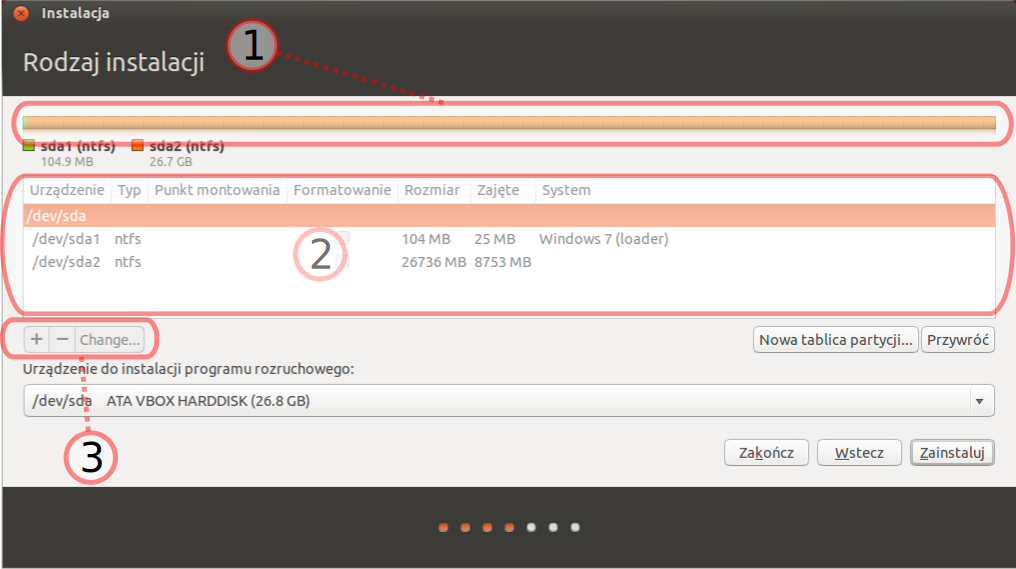
\includegraphics[width=\linewidth]{images/instalator_partycjonowanie_gparted2.png}
\end{center}

Na powyższym obrazku widzisz główne okno programu GParted. Wykryty został układ partycji na dysku twardym. Poziomy pasek \textcolor{ubuntu_orange}{(}1\textcolor{ubuntu_orange}{)} rozciągający się na całą szerokość okna jest graficzną reprezentacją układu partycji. Poniżej paska znajduje się legenda objaśniacza użyte kolory. Tabela \textcolor{ubuntu_orange}{(}2\textcolor{ubuntu_orange}{)} znajdująca się w centralnej części okna przedstawia szczegółowe informacje na temat partycji na dysku twardym. Zestaw przycisków \textcolor{ubuntu_orange}{(}3\textcolor{ubuntu_orange}{)} służy do dodawania partycji (\textcolor{ubuntu_orange}{+}), usuwania partycji (\textcolor{ubuntu_orange}{-}) lub ich modyfikacji(\textcolor{ubuntu_orange}{Change}). Na chwilę obecną inne rzeczy nas nie interesują.

Powyższy układ dysków twardych oraz partycji jest tylko przykładem skonstruowanym na maszynie wirtualnej. Na Twoim komputerze liczby będą inne.
\clearpage
\begin{center}
        \includegraphics[width=\linewidth]{images/instalator_partycjonowanie_gparted2_czysty.png}
\end{center}

Tabela umieszczona w centrum tego okna przedstawia informacje o poszczególnych partycjach obecnych na dysku twardym. Objaśnienie poszczególnych kolumn:
\begin{itemize}
\item \textcolor{ubuntu_orange}{Urządzenie} - Ścieżka do poszczególnych partycji na dysku twardym. Są to oznaczenia stosowane w systemach Uniksowych, do których należy Linux a więc i Ubuntu i opisują jak rozpoznawane są poszczególne partycje. W tym wypadku:
        \begin{itemize}
        \item \textcolor{ubuntu_orange}{/dev/} - skrót od "Device", urządzenie
        \item \textcolor{ubuntu_orange}{sda} - oznaczenie pierwszego dysku twardego.
                \begin{itemize}
                        \item \textcolor{ubuntu_orange}{sd} - dysk na złączu SATA (sata disk)
                        \item \textcolor{ubuntu_orange}{a} - pierwszy dysk. Drugi dysk twardy miałby literę "b", trzeci "c" i tak dalej.
                \end{itemize}
        \item \textcolor{ubuntu_orange}{sda1} - pierwsza partycja na pierwszym dysku twardym.
        \item \textcolor{ubuntu_orange}{sda2} - druga partycja na pierwszym dysku twardym.
        \end{itemize}
\item \textcolor{ubuntu_orange}{Typ} - rodzaj systemu plików. Sposób w jaki partycja została sformatowana. System Windows korzysta z NTFS, Ubuntu może korzystać z różnych.
\item \textcolor{ubuntu_orange}{Punkt montowania} - miejsce w którym dana partycja zostanie "zamontowana", katalog w którym będzie widoczna zawartość tej partycji.
\item \textcolor{ubuntu_orange}{Formatowanie} - zaznaczając to pole informujesz instalator, że dana partycja ma zostać sformatowana. Oznacza to utratę wszystkich danych na niej zapisanych.
\item \textcolor{ubuntu_orange}{Rozmiar} - pojemność partycji w megabajtach.
\item \textcolor{ubuntu_orange}{Zajęte} - ile miejsca zostało zajęte na tej partycji
\item \textcolor{ubuntu_orange}{System} - system operacyjny zainstalowany na danej partycji. Nie zawsze da się rozpoznać zainstalowany system. Nie każda partycja musi mieć zainstalowany system operacyjny. 
\end{itemize}
\clearpage
\subsubsection{Zaawansowane partycjonowanie - Instalacja obok systemu Windows}
\begin{center}
        \includegraphics[width=\linewidth]{images/instalator_partycjonowanie_gparted2_czysty.png}
\end{center}

Na powyższym obrazku widać dwie partycje utworzone przez instalator systemu Windows7. Partycja zielona o rozmiarze 104 megabajtów służy jako partycja dla programu rozruchowego systemu Windows. Duża, pomarańczowa partycja (26736 megabajtów) jest główna partycją systemu Windows7. Bardzo podobny układ partycji stosowany jest przez każdy z systemów z rodziny Windows.\\
Pierwszym krokiem jest zrobienie miejsca dla systemu Ubuntu. Kliknij na partycję \textcolor{ubuntu_orange}{/dev/sda2}. Następnie kliknij na przycisk \textcolor{ubuntu_orange}{Change} znajdujący się pod tabelą. W otwartym oknie możesz zmniejszyć rozmiar wybranej partycji.
\clearpage
\begin{wrapfigure}{R}{0.5\textwidth}
                \includegraphics[width=\linewidth]{images/instalator_partycjonowanie_gparted_zmniejszenie_partycji_windows.png}
\end{wrapfigure}

W polu \textcolor{ubuntu_orange}{Rozmiar} podaj nowy rozmiar partycji. O tym ile miejsca potrzebujesz na Ubuntu przeczytasz w rozdziale \ref{ile_miejsca}: Ile miejsca przeznaczyć na Ubuntu. W polu podajesz rozmiar partycji w megabajtach. Jeden gigabajt to 1024 megabajty.\\
Upewnij się, że wybrano opcję \textcolor{ubuntu_orange}{nie używaj tej partycji}. Teraz kliknij przycisk \textcolor{ubuntu_orange}{OK} a następnie \textcolor{ubuntu_orange}{Naprzód} aby dokonać zmiany na partycji. Wykonanie żądanej zmiany może trwać dłuższą chwilę.
Na schemacie pojawiła się pusta, \textcolor{ubuntu_orange}{dostępna przestrzeń} oznaczona kolorem szarym. Kliknij a nią, a następnie na przycisk (\textcolor{ubuntu_orange}{+}) aby stworzyć nową partycję.

\begin{center}
        \includegraphics[width=\linewidth]{images/instalator_partycjonowanie_gparted3.png}
\end{center}

\clearpage
\begin{wrapfigure}{R}{0.5\textwidth}
                \includegraphics[width=\linewidth]{images/instalator_partycjonowanie_gparted_dodaj_root.png}
\end{wrapfigure}

Po pierwsze musimy stworzyć partycję podstawową dla Ubuntu. O ilości miejsca potrzebnej na poszczególne partycje przeczytasz w sekcji \ref{ile_miejsca}: "Ile miejsca przeznaczyć na Ubuntu". Pozostałe opcje ustaw jak na rysunku.
\begin{itemize}
\item \textcolor{ubuntu_orange}{Rozmiar} - rozmiar partycji w megabajtach
\item \textcolor{ubuntu_orange}{Rodzaj nowej partycji} - jako, że system Windows korzysta z tablicy partycji ms-dos to jesteśmy ograniczeni do 4 partycji podstawowych. Aby nie było problemu, dla Ubuntu utworzymy partycje logiczne.
\item \textcolor{ubuntu_orange}{Lokalizacja dla nowej partycji} - Czy partycja zostanie wyrównana do poczatku wolnej przestrzeni czy do jej końca. Nie ma to znaczenia dla działania systemu.
\item \textcolor{ubuntu_orange}{Użyj jako} - jaki system plików ma być użyty do sformatowania tej partycji. Do wyboru jest wiele, ale w ramach tego przewodnika korzystamy z systemu ext4 z księgowaniem\footnote{Tematyka różnych systemów plików jest bardzo rozległa i z łatwością wypełniłaby kolejny Przewodnik.}
\item \textcolor{ubuntu_orange}{Punkt montowania} - to nasza główna partycja, więc musi się znaleźć na początku\footnote{W systemach Windows drzewo katalogów "zaczyna się" na C:$\backslash\backslash$ W systemach Linuksowych zaczyna się na /}.
\end{itemize}
Kliknij na przycisk \textcolor{ubuntu_orange}{OK} aby utworzyć nową partycję.
\clearpage
\begin{wrapfigure}{R}{0.5\textwidth}
                \includegraphics[width=\linewidth]{images/instalator_partycjonowanie_gparted_dodaj_swap.png}
\end{wrapfigure}
Teraz utwórz partycję wymiany. Więcej o tej partycji przeczytasz w w sekcji \ref{ile_miejsca}: "Ile miejsca przeznaczyć na Ubuntu". Pozostałe opcje ustaw jak na rysunku. Kliknij na przycisk \textcolor{ubuntu_orange}{OK} aby utworzyć nową partycję.
\begin{wrapfigure}{L}{0.5\textwidth}
                \includegraphics[width=\linewidth]{images/instalator_partycjonowanie_gparted_dodaj_home.png}
\end{wrapfigure}
Na koniec pozostało utworzenie partycji domowej. Więcej o tej partycji przeczytasz w w sekcji \ref{ile_miejsca}: "Ile miejsca przeznaczyć na Ubuntu". Pozostałe opcje ustaw jak na rysunku. Kliknij na przycisk \textcolor{ubuntu_orange}{OK} aby utworzyć nową partycję.
\clearpage
\begin{center}
        \includegraphics[width=\linewidth]{images/instalator_partycjonowanie_gparted4.png}
\end{center}
Ekran programu GParted wygląda teraz mniej więcej tak jak na rysunku powyżej. Masz dwie partycje systemu Windows (NTFS), partycję wymiany systemu Linux (swap) oraz dwie partycje dla systemu Ubuntu (ext4). Upewnij się, że partycje NTFS \textcolor{ubuntu_orange}{nie} są zaznaczone do sformatowania, zaś partycje ext4 tak.

Kliknij na przycisk \textcolor{ubuntu_orange}{Naprzód} aby wprowadzić zmiany na partycjach. Teraz możesz powrócić do lektury procesu instalacji w miejscu gdzie go przerwałeś.\\
Powrót do \ref{instalator_strefa_czasowa}: Wybór strefy czasowej.
\clearpage

	\subsection{Rozwiązywanie problemów z instalacją}
		\subsubsection{Po wybraniu opcji ,,Wypróbuj Ubuntu bez instalacji'' lub ,,Instaluj Ubuntu'' mam tylko czarny ekran}
Po pierwsze, nie spiesz się, wczytanie wszystkich danych z nośnika instalacyjnego trwa dłuższą chwilę. Jeżeli nic się nie dzieje dłużej, niż 2 -- 3 minuty, to zrestartuj komputer i uruchom instalator Ubuntu jeszcze raz. W przypadku instalatora BIOS (fioletowe tło) po wybraniu języka wcśnij \keys{F6} (inne opcje), zaznacz opcję ,,nomodeset'' klawiszem \keys{\returnwin}, wyjdź z menu klawiszem \keys{Esc} i uruchom instalator. Opcja ,,acpi=off'' też może być pomocna.

\subsubsection{Instalacja została przerwana}
Jeżeli instalacja została przerwana w trakcie kopiowania danych na dysk, to uruchom ponownie instalator i zainstaluj system od nowa.

Jeżeli instalacja została przerwana w trakcie partycjonowania (zapisywania zmian na dysku), to prawdopodobnie doszło do nieodwracalnego uszkodzenia tablicy partycji. Uruchom nośnik instalacyjny, wybierz ,,Wypróbuj Ubuntu bez instalacji'' (\textit{Try Ubuntu without installing''} i uruchom program GParted.

\subsubsection{Po instalacji Ubuntu uruchamia się tylko Windows}
Prawdopodobnie na Windowsie masz ustawione ,,Szybkie uruchamianie'' (\textit{Fast-boot}). Wyłącz tę funkcję i ponownie zainstaluj Ubuntu. Przeczytaj rozdział \ref{sec:przygotowanie_windows}: ,,Przygotowanie do instalacji''.

\subsubsection{Po instalacji Ubuntu nie można uruchomić systemu Windows}
przyczyny mogą być dwie. Albo usunąłeś system Windows z dysku twardego, albo nie został on prawidłowo rozpoznany. W pierwszym przypadku pozostaje tylko ponownie go zainstalować. Koniecznie przeczytaj rozdział \ref{sec:przygotowanie_windows}: ,,Przygotowanie do instalacji''.

W drugim przypadku przejdź do sekcji ,,Przywracanie GRUB-a''

\subsubsection{Przywracanie GRUB-a}
\label{grub_przywracanie}
Problemy z programem rozruchowym występują najczęściej:
\begin{itemize}
\item Po instalacji systemu Windows obok Ubuntu. Windows nadpisuje MBR (\textit{Master Boot Record)} dysku twardego i uniemożliwia dostęp do systemów linuksowych.
\item Po instalacji Ubuntu obok Windowsa, jeżeli ten był zahibernowany, miał włączoną opcję ,,Fast-Boot'' lub podobne.
\item Po zmianie układu partycji.
\item Po nieumiejętnych próbach edytowania GRUB-a lub zastąpienia go innym menadżerem rozruchowym.
\end{itemize}

Najprostszym sposobem naprawienia menadżera rozruchu GRUB jest skorzystanie z Boot Repair Disk. Jest to dystrybucja Linuksa typu Live (działa tylko z zewnętrznego nośnika, nie zainstalujesz jej na dysku twardym). Otwórz stronę \href{http://sourceforge.net/projects/boot-repair-cd/files/}{pobierania}, wybierz plik z obrazem zgodny z architekturą twojego procesora i zapisz go na dysku. Proces przygotowywania nośnika z Boot Repair Disk jest analogiczny do przedstawionego w rozdziale \ref{nagrywanie_obrazu}: ,,Nagrywanie pobranego obrazu''.\\
Po uruchomieniu tak przygotowanego systemu poczekaj, aż się załaduje i wybierz opcję \textcolor{ubuntu_orange}{Recomended repair}, a nastepnie spróbuj ponownie uruchomić komputer.

Jeżeli nie możesz uruchomić żadnego systemu operacyjnego, to program Boot Repair możesz zainstalować bezpośrednio na nośniku instalacyjnym Ubuntu. Podczas uruchamiania instalatora wybierz ,,Wypróbuj Ubuntu bez instalacji'' (\textit{Try Ubuntu without installing''}, następnie otwórz terminal \keys{CTRL + Alt + t} i wydaj następujące trzy polecenia:

\begin{lstlisting}[language=bash]
sudo add-apt-repository ppa:yannubuntu/boot-repair
sudo sed "s/trusty/saucy/g\" -i /etc/apt/sources.list.d/yannubuntu-boot-repair-trusty.list
sudo apt-get update
sudo apt-get install -y boot-repair && (boot-repair &)
\end{lstlisting}

\subsubsection{Ręczne przywracanie GRUB-a}
Ta metoda jest nieprzydatna, jeżeli masz zainstalowany tylko system Windows.

Jeżeli nie masz możliwości zainstalowania paczek na nośniku instalacyjnym (np. ze względu na brak połączenia z internetem), to możesz spróbować przywrócić GRUB-a ręcznie. Uruchom instalator Ubuntu w trybie ,,Wypróbuj Ubuntu bez instalacji'' (\textit{Try Ubuntu without installing}'', a następnie otwórz terminal \keys{CTRL + Alt + t}.

Zidentyfikuj partycję, na której już jest zainstalowane Ubuntu (lub inny linux). Wykonaj:

\begin{lstlisting}[language=bash]
ls /dev |grep sd
\end{lstlisting}

Otrzymasz listę dysków twardych wraz z partycjami. \textcolor{ubuntu_orange}{sda} to najprawdopodobniej twój główny dysk twardy, sdb to pendrive. Możesz się upewnić wydając polecenie:

\begin{lstlisting}[language=bash]
sudo fdisk -l
\end{lstlisting}

Wyszukaj oznaczenie głównej partycji zainstalowanego linuksa. W wielu przypadkach będzie to /dev/sda1, ale jeżeli masz zainstalowany obok inny system (np. Windows), to może być inaczej. W dalszej częsci tego tekstu zakładamy, że jest to /dev/sda1.

Zamontuj partycję zainstalowanego systemu oraz inne niezbędne rzeczy:
\begin{lstlisting}[language=bash]
sudo mount /dev/sda1 /mnt
sudo mount --bind /dev /mnt/dev
sudo mount --bind /dev/pts /mnt/dev/pts
sudo mount --bind /proc /mnt/proc
sudo mount --bind /sys /mnt/sys
\end{lstlisting}

Przełącz się na nowy system plików:

\begin{lstlisting}[language=bash]
sudo chroot /mnt
\end{lstlisting}

Zainstaluj GRUB-a. Zwróć uwagę, że instalujemy go na dysku (sda), a nie partycji (sda1).

\begin{lstlisting}[language=bash]
grub-install /dev/sda
update-grub
\end{lstlisting}

Wyjdź i posprzątaj po sobie:

\begin{lstlisting}[language=bash]
exit
sudo umount /mnt/sys
sudo umount /mnt/proc
sudo umount /mnt/dev/pts
sudo umount /mnt/dev
sudo umount /mnt
\end{lstlisting}

Teraz ponownie uruchom komputer.
\clearpage

	\subsection{Instalacja na maszynie wirtualnej}
		\begin{wrapfigure}{R}{0.5\textwidth}
                \includegraphics[width=\linewidth]{images/virtualbox_download.png}
\end{wrapfigure}

Alternatywnym sposobem wypróbowania Ubuntu bez instalowania go na dysku twardym jest wykorzystanie maszyny wirtualnej. Oprogramowanie to umożliwia uruchomienie jednego systemu wewnątrz drugiego. Wiąże się to oczywiście z dużym zapotrzebowaniem na moc obliczeniową procesora oraz pamięć operacyjną. Jeżeli masz przynajmniej 2 gigabajty RAMu a twój procesor jest nie starszy niż 5 lat (wtedy jest szansa, że będzie zapewniał akcelerację sprzętową dla wirtualizacji) to możesz w ten sposób wypróbować Ubuntu.

Udaj się na stronę \href{https://www.virtualbox.org/wiki/Downloads}{virtualbox.org/download} i pobierz instalator Virtualboksa dla swojego systemu. Zainstaluj pobrany plik w swoim systemie i uruchom program Virtualbox.
\clearpage
\begin{center}
        \includegraphics[scale=0.7]{images/virtualbox_main.png}
\end{center}

W oknie głównym programu Virtualbox kliknij na przycisk \textcolor{ubuntu_orange}{New} aby uruchomić kreator maszyny wirtualnej.
\clearpage
\begin{wrapfigure}{r}{0.5\textwidth}
                \includegraphics[width=\linewidth]{images/virtualbox_wizard1.png}
\end{wrapfigure}

\begin{itemize}
\item \textcolor{ubuntu_orange}{Name} - Nazwa maszyny wirtualne. Może to być cokolwiek.
\item \textcolor{ubuntu_orange}{Type} - Typ systemu. Ustaw na \textcolor{ubuntu_orange}{Linux}
\item \textcolor{ubuntu_orange}{Version} - Wersja systemu. Ustaw na \textcolor{ubuntu_orange}{Ubuntu (64 bit)}.\\
Uwaga: Architektura wybranego systemu (32/64 bit) musi być zgodna z architekturą twojego procesora. Jeżeli posiadasz 64 bitowy procesor ( najprawdopodobniej posiadasz, jeżeli twój komputer nie jest starszy niż 6 lat) to wybierz system 64 bitowy. Pamiętaj też, że pobrany obraz instalatora Ubuntu też musi odpowiadać tej architekturze.
\end{itemize}
\begin{flushright}
Kliknij na przycisk \textcolor{ubuntu_orange}{Next} aby przejść dalej.
\end{flushright}

\clearpage
\begin{wrapfigure}{r}{0.5\textwidth}
                \includegraphics[width=\linewidth]{images/virtualbox_wizard2.png}
\end{wrapfigure}

Na tym ekranie ustaw ilość pamięci operacyjnej twojego komputera jaką chcesz przeznaczyć dla systemu-gościa. Weź pod uwagę, że ta pamięć zostanie zajęta w momencie uruchomienia maszyny wirtualnej i nie będzie dostępna dla systemu-gospodarza. Nie powinno się przydzielać gościowi więcej niż 50\% zasobów gospodarza. Ubuntu wymaga minimum 512 megabajtów (system plus oprogramowanie) a zdecydowanie lepiej jest przydzielić 1024 megabajty.
Jeżeli w twoim komputerze jest zainstalowane tylko 2 gigabajty RAMu to przydzielając 1 gigabajt gościowi pozostanie ci tylko 1 gigabajt dla gospodarza. Nie jest to dobre rozwiązanie, gdyż prawdopodobnie będziesz musiał wyłączyć większość programów na systemie gospodarza aby nie doszło do przepełnienia pamięci operacyjnej. Prawie na pewno będziesz musiał wyłączyć przeglądarkę internetową. 
\begin{flushright}
Kliknij na przycisk \textcolor{ubuntu_orange}{Next} aby przejść dalej.
\end{flushright}
\clearpage
\begin{wrapfigure}{r}{0.5\textwidth}
                \includegraphics[width=\linewidth]{images/virtualbox_wizard3.png}
\end{wrapfigure}

Ten ekran pozwala stworzyć wirtualny dysk twardy lub stworzyć nowy. Na tym etapie nie masz żadnego takiego urządzenia a wiec wybierz środkowa opcję \textcolor{ubuntu_orange}{Create a virtual hard drive now}.
\begin{flushright}
Kliknij na przycisk \textcolor{ubuntu_orange}{Next} aby przejść dalej.
\end{flushright}
\clearpage
\begin{wrapfigure}{r}{0.5\textwidth}
                \includegraphics[width=\linewidth]{images/virtualbox_wizard4.png}
\end{wrapfigure}

Na tym ekranie wybierz typ dysku twardego. Wybierz opcję \textcolor{ubuntu_orange}{VDI (Virtual Disk Image)}.
\begin{flushright}
Kliknij na przycisk \textcolor{ubuntu_orange}{Next} aby przejść dalej.
\end{flushright}
\clearpage
\begin{wrapfigure}{r}{0.5\textwidth}
	\includegraphics[width=\linewidth]{images/virtualbox_wizard5.png}
\end{wrapfigure}

Wybierz pomiędzy dyskiem tworzonym dynamicznie a dyskiem o stałym rozmiarze.
\begin{itemize}
\item \textcolor{ubuntu_orange}{Dynamically allocated} - Taki wirtualny dysk twardy nie zajmuje całego przydzielonego miejsca a jedynie tyle ile wynosi suma rozmiaru plików na nim zapisanych. Nawet jeżeli stworzysz dysk o pojemności 100 gigabajtów, to po instalacji Ubuntu będzie on zajmował tylko trochę ponad 6 gigabajtów na systemie-gospodarzu. Wybierz tą opcję.
\item \textcolor{ubuntu_orange}{Fixed size} - Taki dysk twardy zawsze zajmuje tyle miejsca na systemie-gospodarzu ile zostało zadeklarowane. Jeżeli stworzysz 100 gigabajtowy dysk wirtualny, to na twoim komputerze pojawi się 100 gigabajtowy plik z maszyną wirtualną. Tworzenie takiego dysku też trwa dłuższą chwilę, gdyż dużo danych musi zostać zapisanych na dysk.
\end{itemize}
\begin{flushright}
Kliknij na przycisk \textcolor{ubuntu_orange}{Next} aby przejść dalej.
\end{flushright}
\clearpage
\begin{wrapfigure}{r}{0.5\textwidth}
                \includegraphics[width=\linewidth]{images/virtualbox_wizard6.png}
\end{wrapfigure}

Na tym ekranie możesz wybrać rozmiar dysku twardego. Korzystając z suwaka możesz wybrać żądany rozmiar. Ubuntu 14.04 LTS wymaga przynajmniej 6.2 gigabajta, górną granicą są tylko możliwości Virtualboksa (2 terabajty). W celach testowych stwórz dysk o rozmiarze przynajmniej 25 gigabajtów.

Kliknij na przycisk \textcolor{ubuntu_orange}{Create} aby stworzyć dysk i zakończyć działanie kreatora.

\clearpage
\begin{center}
	\includegraphics[width=\linewidth]{images/virtualbox_start.png}
\end{center}

Twoja maszyna wirtualna dla Ubuntu jest gotowa. W głównym oknie programu Virtualbox jest teraz dostępna. Kliknij na nią i z paska narzędziowego wybierz \textcolor{ubuntu_orange}{Start}. Alternatywnym sposobem uruchomienia maszyny wirtualnej jest dwukrotne kliknięcie na jej ikonie. Twoim oczom ukaże się okno jak na rysunku powyżej. Kliknij na żółtą ikonę folderu i wskaż pobrany wczesnej obraz instalatora systemu Ubuntu (plik .iso). Kliknij \textcolor{ubuntu_orange}{Start} aby uruchomić maszynę wirtualną. Instalacja na maszynie wirtualnej przebiega tak samo jak w rzeczywistości. Przejdź do sekcji \ref{instalacja_uruchomienie}: "Uruchomienie instalatora BIOS".

Kiedy po zakończeniu instalacji zostaniesz poproszony o wyjście płyty instalatora z napędu to z paska menu maszyny wirtualnej wybierz Devices Cd/DVD Devices Remove disk from virtual drive.
\clearpage
		
\section{Pierwsze uruchomienie systemu}
	\label{sec:pierwsze_uruchomienie}
	\subsection{Proces uruchamiania systemu}
		\begin{wrapfigure}{R}{0.5\textwidth}
		\includegraphics[width=\linewidth]{images/pierwsze_uruchomienie_grub.png}
\end{wrapfigure}

Po zainstalowaniu systemu Ubuntu twój komputer został zresetowany.
\clearpage
	\subsection{Ekran logowania}
	\subsection{Rzut oka na Pulpit Ubuntu}
	\subsection{Rzeczy do zrobienia po instalacji Ubuntu}
		\label{sec:rzeczy_do_zrobienia_po_instalacji}
		%Aktualizacja systemu, zmiana tapety 
		%instalacja sterowników
		%instalacja kodeków (ubuntu restricted extras) i spolszczenia
		%Instalacja flasha
		%pakiety unzip, unrar, p7zip-full
\section{Pulpit Ubuntu Unity}
	\subsection{Pulpit}
		%Pulpit, zmiana tapety tworzenie wyzwalaczy, wirtualne pulpity
	\subsection{Zarządzanie oknami}
	\subsection{Panel Menu}
		%Global menu, wskaźniki, notufikacje
	\subsection{Launcher}
		%Modyfikowanie i tworzenie nowych
	\subsection{Dash}
	\subsection{HUD}
	\subsection{Nautilus}
	\subsection{Totem}
	\subsection{Rhythmbox}
	\subsection{Firefox}
	\subsection{Evolution}
	\subsection{LibreOffice}
	\subsection{Konta online}
	\subsection{Centrum Oprogramowania}
\section{Sztuczki z systemem Ubuntu}
	\subsection{Prywatność}
	\subsection{Zmiana położenie elementów sterujących okna}
	\subsection{Click to minimize}
	\subsection{Wyłączenie global menu}
	\subsection{Instalacja nowych motywów graficznych}
	
\end{document}
